\documentclass[11pt,a4paper]{article}

\usepackage[margin=2.8cm]{geometry}
\usepackage[T1]{fontenc}
\usepackage[utf8]{inputenc}
\usepackage{lmodern}
\usepackage{graphicx}
\usepackage{booktabs}
\usepackage{tabularx}
\usepackage{longtable}
\usepackage{enumitem}
\usepackage{xcolor}
\usepackage{url}
\usepackage[round,authoryear]{natbib}

\newcommand{\parencite}[1]{\citep{#1}}

\graphicspath{{../papers/arxiv-1612.03770v2/}{figures/}}

\setlist[itemize]{leftmargin=*,topsep=0.35em,itemsep=0.25em}
\setlist[enumerate]{leftmargin=*,topsep=0.35em,itemsep=0.25em}
\newcommand{\todoresult}[1]{\textcolor{red}{TODO(result): #1}}
\newcommand{\todocite}[1]{\textcolor{orange}{TODO(cite): #1}}
\newcommand{\artifact}[1]{\path{#1}}

\title{Replication Protocol: Neurogenesis Deep Learning and Dynamic-Capacity Neural Architectures}
\author{Replication notes}
\date{\today}

\begin{document}
\maketitle

\begin{abstract}
This protocol documents a replication of Neurogenesis Deep Learning (NDL) and a literature review on neural network architectures that change size during training. The first part describes the original method, the local implementation, and the experimental protocol. The second part organizes related work by architecture-change mechanism: growth, continual-learning expansion, pruning, grow-prune cycles, dynamic sparse rewiring, and architecture morphism. The document is intentionally written as citation-bearing bullet notes so that each point can later be expanded into prose.
\end{abstract}

\tableofcontents
\clearpage

\section{Introduction and Research Questions}

\subsection{Problem and motivation}
\begin{draftpoints}
  \item \draftkey{Problem}new-class acquisition without degradation of earlier representations; fixed-capacity stability--plasticity conflict
  \item \draftkey{NDL premise}excessive reconstruction error $\rightarrow$ insufficient capacity $\rightarrow$ new neurons at the affected depth \parencite{draelos2017neurogenesis}
  \item \draftkey{Primary outcomes}macro reconstruction MSE; foreground-pixel MSE; positive forgetting; architecture growth; computational cost; no classification-accuracy substitute
  \item \draftkey{Controlled question}dynamic-capacity advantage after matching replay, endpoint parameters, optimization effort, and cap effects
\end{draftpoints}

\subsection{Confirmatory research questions}
\begin{draftpoints}
  \item \draftkey{RQ1: fidelity}error detection $\rightarrow$ insertion $\rightarrow$ local plasticity $\rightarrow$ replay stabilization $\rightarrow$ next-layer propagation \parencite{draelos2017neurogenesis}
  \item \draftkey{RQ2: growth}NDL versus exact endpoint-capacity-matched CL; identical replay regime
  \item \draftkey{RQ3: replay}none versus original data versus intrinsic; acquisition, retention, growth demand, final quality
  \item \draftkey{RQ4: organic capacity}quota-satisfied stops versus exhausted class/stream allowances
  \item \draftkey{RQ5: robustness}optimizer; threshold; phase length; outlier quota; geometry; early stopping; global coupling
  \item \draftkey{RQ6: transfer}MNIST ordering versus larger NIST SD-19 feasibility result
\end{draftpoints}

\subsection{Exploratory and qualitative questions}
\begin{draftpoints}
  \item \draftkey{RQ7: training behavior}incoming-class acquisition; old-class retention; updates spent; unresolved outliers
  \item \draftkey{RQ8: visual quality}aggregate MSE versus recognizable base-, early-, and late-class reconstructions
  \item \draftkey{RQ9: later mechanisms}predictive coding; post-class global coupling; stability--plasticity change
\end{draftpoints}

\subsection{Scope and evidential boundaries}
\begin{draftpoints}
  \item \draftkey{Confirmatory boundary}paper-shaped NDL and capacity-matched CL only; predictive coding and global coupling = extensions
  \item \draftkey{Preserved evidence}complete seed-level and per-class exports; incomplete checkpoints and raw logs; stronger endpoint than trajectory claims
  \item \draftkey{Original-data boundary}several graphical-only outcomes; directional comparison unless machine-readable values exist
\end{draftpoints}

\section{Original NDL Paper}

\subsection{Core method}
\begin{itemize}
  \item NDL frames new-class learning as a capacity-allocation problem: when a trained model encounters samples that are poorly represented, it should add new neurons rather than only update existing weights \parencite{draelos2017neurogenesis}.
  \item The original architecture uses stacked autoencoders, which expose layer-wise reconstruction error and therefore provide a local signal for detecting representational bottlenecks \parencite{draelos2017neurogenesis}.
  \item New neurons are inserted into the layer where reconstruction error indicates insufficient capacity, making NDL a growth-only, neuron-level, layer-local architecture-change method.
  \item The method is biologically motivated by neurogenesis, but the implemented mechanism is engineering-oriented: monitor reconstruction quality, add units, and retrain affected parameters.
\end{itemize}

\subsection{Original experimental setting}
\begin{itemize}
  \item The original experiments use incremental visual classification settings, including MNIST-style and NIST SD-19-style digit/class learning tasks \parencite{draelos2017neurogenesis}.
  \item The relevant comparison is not only NDL versus conventional learning, but also the interaction between growth and replay-like mechanisms.
  \item Original figures from the arXiv source bundle are available in \artifact{docs/papers/arxiv-1612.03770v2/} and can be reused when explaining the paper architecture and reported results.
\end{itemize}

\subsection{Claims to verify in the replication}
\begin{itemize}
  \item NDL should help when new classes introduce patterns that the current representation cannot encode well.
  \item Intrinsic replay or replay-based stabilization should be evaluated separately because replay can reduce forgetting independently of architecture growth.
  \item The replication should report both predictive performance and structural side effects, especially hidden-layer size changes and total parameter growth.
\end{itemize}

\begin{figure}[htbp]
  \centering
  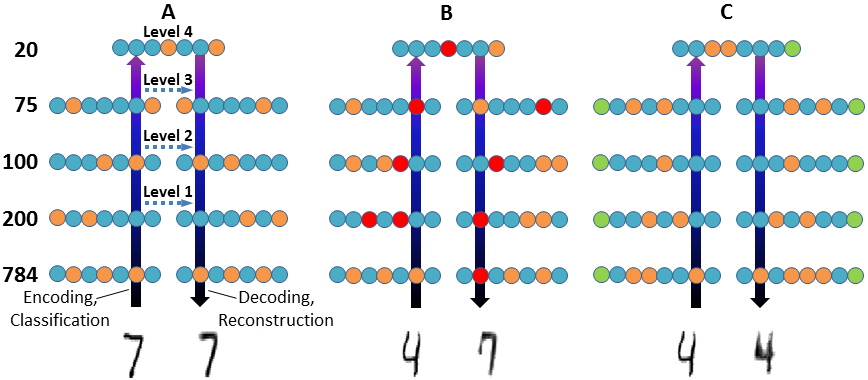
\includegraphics[width=0.78\linewidth]{Figure1.png}
  \caption{Original paper figure placeholder from the arXiv source bundle. Replace or relabel with the most relevant original architecture figure during final writing.}
  \label{fig:original-paper-placeholder}
\end{figure}

\section{Replication Implementation}

\subsection{Repository structure}
\begin{itemize}
  \item The replication is implemented as a configurable Python project with source code under \artifact{src/}, experiment definitions under \artifact{config/}, and paper-level scripts under \artifact{scripts/}.
  \item The original paper source is preserved under \artifact{docs/papers/arxiv-1612.03770v2/}, which allows the report to compare local implementation choices against the paper text and figures.
  \item The dynamic-capacity literature overview is stored as \artifact{docs/papers/dynamic_capacity_taxonomy_original_figures_cl.html}; it should be treated as a local taxonomy draft, not as a citable scholarly source.
\end{itemize}

\subsection{Implemented experiment families}
\begin{itemize}
  \item \artifact{scripts/run_paper_experiments.py} defines a compact paper suite covering MNIST classical learning, MNIST classical learning with intrinsic replay, MNIST NDL, MNIST NDL with intrinsic replay, and SD-19 NDL variants.
  \item \artifact{scripts/run_paper_config.py} runs YAML-defined paper experiments from \artifact{config/paper/}, supports repeated runs, assigns seeds, logs to MLflow when available, and writes summary artifacts.
  \item The key paper configurations are \artifact{mnist_cl}, \artifact{mnist_cl_ir}, \artifact{mnist_ndl}, \artifact{mnist_ndl_ir}, \artifact{sd19_ndl}, \artifact{sd19_ndl_ir}, and \artifact{figure4}.
\end{itemize}

\subsection{Implementation claims to document}
\begin{itemize}
  \item Classical learning baselines isolate the effect of ordinary parameter updates without architecture growth.
  \item Intrinsic replay baselines isolate the effect of replay without architecture growth.
  \item NDL runs isolate the effect of neurogenesis-style hidden-layer growth.
  \item NDL with replay evaluates whether growth and replay act as complementary mechanisms.
  \item SD-19 variants test whether the implementation generalizes beyond the smaller MNIST setting.
\end{itemize}

\subsection{Implementation evidence to include}
\begin{itemize}
  \item Record the exact command used for each run, including the config file path and seed policy.
  \item Record the final hidden sizes and total parameter counts because architecture growth is the central treatment.
  \item Record update counts for pretraining, neurogenesis, incremental training, and the full run when the summary JSON exposes them.
  \item Record runtime and hardware environment as reproducibility metadata rather than as the main result.
\end{itemize}

\section{Experimental Protocol}

\subsection{Main paper experiments}
\begin{itemize}
  \item \artifact{mnist_cl}: MNIST, conventional learning, replay disabled; conventional baseline.
  \item \artifact{mnist_cl_ir}: MNIST, conventional learning with intrinsic replay; replay-only comparison.
  \item \artifact{mnist_ndl}: MNIST, neurogenesis without replay; growth-only comparison.
  \item \artifact{mnist_ndl_ir}: MNIST, neurogenesis with intrinsic replay; growth plus replay.
  \item \artifact{sd19_ndl}: SD-19, neurogenesis with dataset replay mode; larger dataset comparison.
  \item \artifact{sd19_ndl_ir}: SD-19, neurogenesis with dataset replay mode; larger dataset comparison with replay condition.
\end{itemize}

\subsection{Figure 4 replication}
\begin{itemize}
  \item The \artifact{config/paper/figure4.yaml} experiment compares CL, NDL, CL+IR, and NDL+IR on MNIST.
  \item The configured repetition count is five, with sequential seeds starting from 42.
  \item This experiment should be the main source for a replicated Figure 4-style result once outputs are available.
\end{itemize}

\subsection{Ablation experiments}
\begin{itemize}
  \item Growth-shape ablation: test whether the rule for distributing added capacity affects performance or parameter efficiency.
  \item Funnel-shape ablation: test whether hidden-layer geometry affects reconstruction bottlenecks and growth behavior.
  \item Global-coupling ablation: test whether local growth decisions need stronger global coordination.
  \item Outlier-quota ablation: test whether growth is robust to thresholding or quota choices for poorly reconstructed samples.
  \item Early-stop ablation: test whether training duration and stopping rules materially change the comparison between regimes.
  \item Training-protocol ablation: test whether the replication conclusions depend on scheduling and optimization details.
\end{itemize}

\subsection{Reproducibility checklist}
\begin{itemize}
  \item Environment files: \artifact{environment.yml}, \artifact{pyproject.toml}, and \artifact{setup.py}.
  \item Main command pattern:
    \begin{quote}
      \small\texttt{python scripts/run\_paper\_config.py}\\
      \small\texttt{-{}-config config/paper/figure4.yaml}
    \end{quote}
  \item Single-suite command pattern:
    \begin{quote}
      \small\texttt{python scripts/run\_paper\_experiments.py}\\
      \small\texttt{-{}-output outputs/paper\_experiments\_summary.json}
    \end{quote}
  \item Required result artifacts: summary JSON, plotted comparison figure, MLflow run metadata if available, and final trained-model structural statistics.
  \item Hardware metadata: \todoresult{add CPU/GPU, RAM, operating system, Python version, and package environment used for the final runs.}
\end{itemize}

\section{Results}

\subsection{Available result status}
\begin{itemize}
  \item No result artifacts were visible in the workspace during protocol drafting, so numeric claims must remain placeholders until the experiments are run or external outputs are copied into the project.
  \item All result statements below are structured as slots: each one must be replaced by measured values, linked tables, or generated figures before final submission.
\end{itemize}

\subsection{Main MNIST comparison}
\begin{itemize}
  \item CL baseline: \todoresult{insert final accuracy, forgetting metric if available, hidden sizes, and runtime.}
  \item CL+IR baseline: \todoresult{insert final accuracy and compare against CL to isolate replay effect.}
  \item NDL without replay: \todoresult{insert final accuracy and compare against CL to isolate architecture-growth effect.}
  \item NDL+IR: \todoresult{insert final accuracy and compare against all other MNIST regimes to estimate combined growth/replay effect.}
  \item Interpretation bullet: if NDL+IR outperforms CL+IR, the replication supports a contribution from architecture growth beyond replay; if not, the result suggests replay explains most of the benefit.
\end{itemize}

\subsection{SD-19 comparison}
\begin{itemize}
  \item SD-19 NDL: \todoresult{insert final accuracy, hidden sizes, total parameter count, and runtime.}
  \item SD-19 NDL+IR: \todoresult{insert final accuracy and compare with SD-19 NDL.}
  \item Interpretation bullet: SD-19 should be discussed as a harder scalability check because it better tests whether growth rules remain useful outside the MNIST replication.
\end{itemize}

\subsection{Architecture growth and efficiency}
\begin{itemize}
  \item Hidden-layer growth table: \todoresult{insert initial hidden sizes, final hidden sizes, and number of added neurons per layer.}
  \item Parameter-efficiency table: \todoresult{insert total parameters and accuracy per parameter for each regime.}
  \item Runtime table: \todoresult{insert runtime and update-count metrics to separate accuracy gains from compute cost.}
  \item Interpretation bullet: growth should be reported as both a learning mechanism and a cost because dynamic capacity can improve plasticity while increasing memory and compute.
\end{itemize}

\subsection{Ablation summary}
\begin{itemize}
  \item Growth-shape ablation: \todoresult{insert best/worst growth-shape condition and measured effect.}
  \item Funnel-shape ablation: \todoresult{insert whether funnel geometry changes growth frequency or accuracy.}
  \item Global-coupling ablation: \todoresult{insert whether local layer decisions require global coordination.}
  \item Outlier-quota ablation: \todoresult{insert sensitivity to quota or threshold choices.}
  \item Early-stop ablation: \todoresult{insert whether stopping criteria alter the qualitative conclusion.}
  \item Training-protocol ablation: \todoresult{insert whether optimization schedule changes the replication outcome.}
\end{itemize}

\section{Literature Review: Size-Changing ANN Architectures}

\subsection{Taxonomy used for the review}
\begin{itemize}
  \item Dynamic-capacity methods can be organized by what changes: neurons, channels, layers, modules, weights, masks, or architecture paths.
  \item They can also be organized by trigger signal: reconstruction error, residual error, task boundary, gradient signal, orthogonality, sparsity penalty, or architecture search.
  \item NDL belongs to the growth-only branch: it adds neurons at layer-local bottlenecks indicated by reconstruction error \parencite{draelos2017neurogenesis}.
  \item The local HTML overview in \artifact{docs/papers/dynamic_capacity_taxonomy_original_figures_cl.html} should guide the structure, while Zotero-managed papers should provide the citable evidence.
\end{itemize}

\subsection{Constructive and growth-only networks}
\begin{itemize}
  \item Cascade-Correlation is an early constructive neural-network method that starts with a small network and adds hidden units when residual error indicates that the current architecture is insufficient \parencite{fahlman1990cascade}.
  \item NDL extends the constructive-network idea into a deep representation-learning setting by using reconstruction error inside a stacked autoencoder hierarchy \parencite{draelos2017neurogenesis}.
  \item Modern growth methods such as GradMax select new units using gradient-based criteria, replacing NDL's reconstruction-error trigger with an optimization-local growth signal \parencite{evci2022gradmax}.
  \item Orthogonality-based expansion methods such as NORTH* use activation- or weight-orthogonality triggers to decide when, where, and how many neurons to add \parencite{maile2022north}.
\end{itemize}

\subsection{Continual-learning expansion}
\begin{itemize}
  \item Progressive Neural Networks avoid catastrophic forgetting by freezing old columns and adding new task-specific columns, making expansion a direct forgetting-control mechanism \parencite{rusu2016progressive}.
  \item Dynamically Expandable Networks add capacity when a new task cannot be represented well by the existing model, combining expansion with selective retraining and regularization \parencite{yoon2018den}.
  \item DER treats representation size as task-adaptive and links growth to continual-learning stability \parencite{yan2021der}.
  \item PathNet searches or selects paths through a larger modular network, using architectural routing rather than simple neuron insertion \parencite{fernando2017pathnet}.
  \item Learn-to-Grow-style methods choose how much sharing or expansion is needed between tasks, making the architecture decision itself part of continual learning \parencite{li2019learn}.
\end{itemize}

\subsection{Pruning and removal}
\begin{itemize}
  \item Magnitude pruning removes low-importance weights after or during training, changing capacity by deletion rather than growth \parencite{han2015deep}.
  \item Dynamic Network Surgery alternates pruning and splicing so that mistakenly removed connections can be restored \parencite{guo2016dynamic}.
  \item Network Slimming learns channel-level scale factors and removes channels with low importance, producing structured smaller networks that map better to dense hardware \parencite{liu2017network}.
  \item L0 regularization uses learned gates to induce sparsity, integrating removal pressure into the objective rather than applying pruning only as a post-processing step \parencite{louizos2018learning}.
\end{itemize}

\subsection{Grow-prune systems}
\begin{itemize}
  \item NeST combines growth and pruning to search for compact architectures, making capacity change bidirectional rather than growth-only \parencite{dai2018nest}.
  \item MorphNet learns resource-aware architecture changes and can shrink or expand networks under computational constraints \parencite{gordon2018morphnet}.
  \item Grow-prune systems are useful comparison points for NDL because they treat added capacity as provisional and later remove unnecessary structure.
\end{itemize}

\subsection{Dynamic sparse training and rewiring}
\begin{itemize}
  \item Sparse Evolutionary Training trains sparse networks while periodically rewiring connections, keeping active parameter count constrained while changing topology \parencite{mocanu2018scalable}.
  \item RigL uses gradient information to regrow sparse connections, making rewiring more targeted than random sparse evolution \parencite{evci2020rigging}.
  \item Sparse rewiring differs from NDL because it usually preserves a fixed active-parameter budget rather than monotonically increasing capacity.
\end{itemize}

\subsection{Architecture morphism and search}
\begin{itemize}
  \item Net2Net widens or deepens networks using function-preserving transformations, giving larger models a stable initialization that initially preserves old behavior \parencite{chen2016net2net}.
  \item Network morphism and transformation-based architecture search generalize this idea by modifying architecture while trying to preserve function or training progress \parencite{wei2016network}.
  \item Differentiable architecture search methods optimize over architecture choices rather than reacting to reconstruction or residual errors \parencite{liu2019darts}.
  \item Architecture morphism is an important contrast to NDL because it emphasizes safe transformation of a trained function, while NDL emphasizes local growth triggered by poor representation.
\end{itemize}

\subsection{Synthesis for the protocol}
\begin{itemize}
  \item NDL is best positioned as an early deep-learning example of local, error-triggered, growth-only dynamic capacity.
  \item Its main strength is interpretability of the growth trigger inside autoencoder layers; its main limitation is dependence on reconstruction modules, which do not directly exist in ordinary classifiers, CNNs, or transformer architectures.
  \item Later literature broadens the design space along four axes: safer initialization, stronger forgetting protection, resource-aware pruning, and sparse/topological adaptation.
  \item The final discussion should evaluate whether the replication suggests that NDL's specific reconstruction-error trigger remains compelling compared with later gradient-, task-, sparsity-, or search-driven triggers.
\end{itemize}

\subsection{Zotero management notes}
\begin{itemize}
  \item Use a Zotero group or collection named \artifact{Neurogenesis} for the selected literature set.
  \item Use Better BibTeX to export the selected references to \artifact{docs/protocol/references.bib}.
  \item Run the Zotero sync workflow in dry-run mode before importing missing entries, then rerun without dry-run only for missing citekeys.
  \item Keep citekeys stable because section bullets already refer to them.
\end{itemize}

\section{Discussion and Next Writing Steps}

\subsection{Expected interpretation structure}
\begin{itemize}
  \item Start by separating the effects of replay, growth, and their combination; otherwise the replication may over-attribute improvements to neurogenesis when replay is responsible.
  \item Discuss performance and architecture size together because a dynamic-capacity method can improve accuracy by spending more parameters.
  \item Treat SD-19 results as the stronger external-validity check and MNIST results as the controlled replication anchor.
  \item Use ablations to identify whether the implementation conclusion depends on thresholding, growth geometry, global coupling, stopping rules, or training schedule.
\end{itemize}

\subsection{Limitations to state explicitly}
\begin{itemize}
  \item If only MNIST results are available, the replication should be described as partial and small-scale.
  \item If result variance across seeds is large, conclusions should be stated in terms of trends rather than definitive ranking.
  \item If NDL improves accuracy but grows substantially, the report should state the cost rather than only the gain.
  \item If the local implementation differs from the original paper in training schedule, replay implementation, or dataset preprocessing, those differences should be listed before interpreting discrepancies.
\end{itemize}

\subsection{Conversion from bullets to prose}
\begin{itemize}
  \item Convert each bullet into one short paragraph.
  \item Keep citations attached to the claim they support.
  \item Replace every result TODO marker with a table value, figure reference, or explicit statement that the experiment was not run.
  \item Replace any placeholder citation only after the corresponding Zotero entry has been verified in \artifact{references.bib}.
\end{itemize}


\bibliographystyle{plainnat}
\bibliography{references}

\end{document}
